
%(BEGIN_QUESTION)
% Copyright 2006, Tony R. Kuphaldt, released under the Creative Commons Attribution License (v 1.0)
% This means you may do almost anything with this work of mine, so long as you give me proper credit

The sample valve in a gas chromatograph plays an extremely important role: it must inject a precise volume of sample gas to be analyzed, in a precise amount of time.  The following diagram shows the components of a basic gas chromatograph.  Liquid chromatographs differ only slightly from this:

$$\includegraphics[width=15.5cm]{i00675x01.eps}$$

Given the importance of this function, the sample valve is constructed quite differently from ordinary valves.  Most chromatograph sample valves are rotary in nature, with slots cut into a metal rotor for directing fluid flows along different paths.  A common sample valve design uses six ports and three slots, like this:

$$\includegraphics[width=15.5cm]{i00675x03.eps}$$

The following illustration shows a typical sample valve with a rotary valve element, in two different positions.  The {\it loading} position prepares the sample loop for injection while the column is flushed with carrier gas.  The {\it sampling} position injects a precise volume of sample into the column followed by carrier gas.

$$\includegraphics[width=15.5cm]{i00675x02.eps}$$

Explain how this valve and tubing arrangement provides a consistent, measured sample volume during each injection cycle.  Also, identify what would have to change in order to double the amount of injected volume into the column for each injection cycle.

\underbar{file i00675}
%(END_QUESTION)





%(BEGIN_ANSWER)

The injected volume for a chromatograph's sample is determined by the internal volume of the sample loop tubing {\it plus} the volume of one valve slot.  Thus, to exactly double the injected volume, one must increase the sample loop tube length by a factor of a little more than two.

\vskip 10pt

Process chromatographs use very small sample volumes.  To put things into perspective, the typical sample volume for a chromatograph is in the order of tens of {\it micro}-liters! 

\vskip 10pt

The amount of time the sample valve spends in the sampling position has no effect whatsoever on the injected sample volume {\it so long as it exceeds the minimum amount of time required to completely flush the sample loop and valve slot of their contained volumes.}  Any time greater than this is irrelevant.  If the valve spends less than this minimum amount of time in the sampling position, however, the sample loop will not get completely emptied of sample, and the injected sample volume will be less than desired.

%(END_ANSWER)





%(BEGIN_NOTES)


%INDEX% Measurement, analytical: chromatography

%(END_NOTES)


